\section{Avalização da solução Escalável}

Para a avaliação da solução prosposta, realizou-se a implantação dos componentes do \textit{kubernetes} descritos na Seção anterior em um \textit{cluster}, hospedado no provedor DigitalOcean, composto por cinco máquinas com 2 vCPUs e 4 GB de memória RAM cada, onde uma das máquinas atua como \textit{control plane} e os demais quatro funcionam como \textit{nodes}.

Assim como apresentado na Seção 3, para simulação de carga foi utilizado o \textit{Apache HTTP server benchmarking}. 

\subsection{Experimento Inicial}

Inicialmente, foram realizados 10 lotes de teste para cada configuração de cenário, sendo cada lote composto pela realização de 200 requisições ao serviço de autenticação de usuário do \textit{Metabase}. Considera-se uma configuração de cenário, a definição de um parâmentro de concorrência, que define a quantidade de requisições simultâneas ao serviço, e uma quantidade de \textit{pods}, ou seja, instâncias em execução. O parâmetro de concorrência foi variado de 1 a 60, em passos de 10, e a quantidade de instâncias variou de 1 a 4, resultando assim em 28 cenários distintos.

Os resultados dos cenários de teste descritos acima pode ser visto na Figura \ref{fig.avg-resp-time-cluster}, onde cada linha representa uma quantidade distinta de instâncias e cada ponto da linha representa a média do tempo de resposta para cada um dos parâmetros de concorrência.

\begin{figure}[htp]
   \centering
    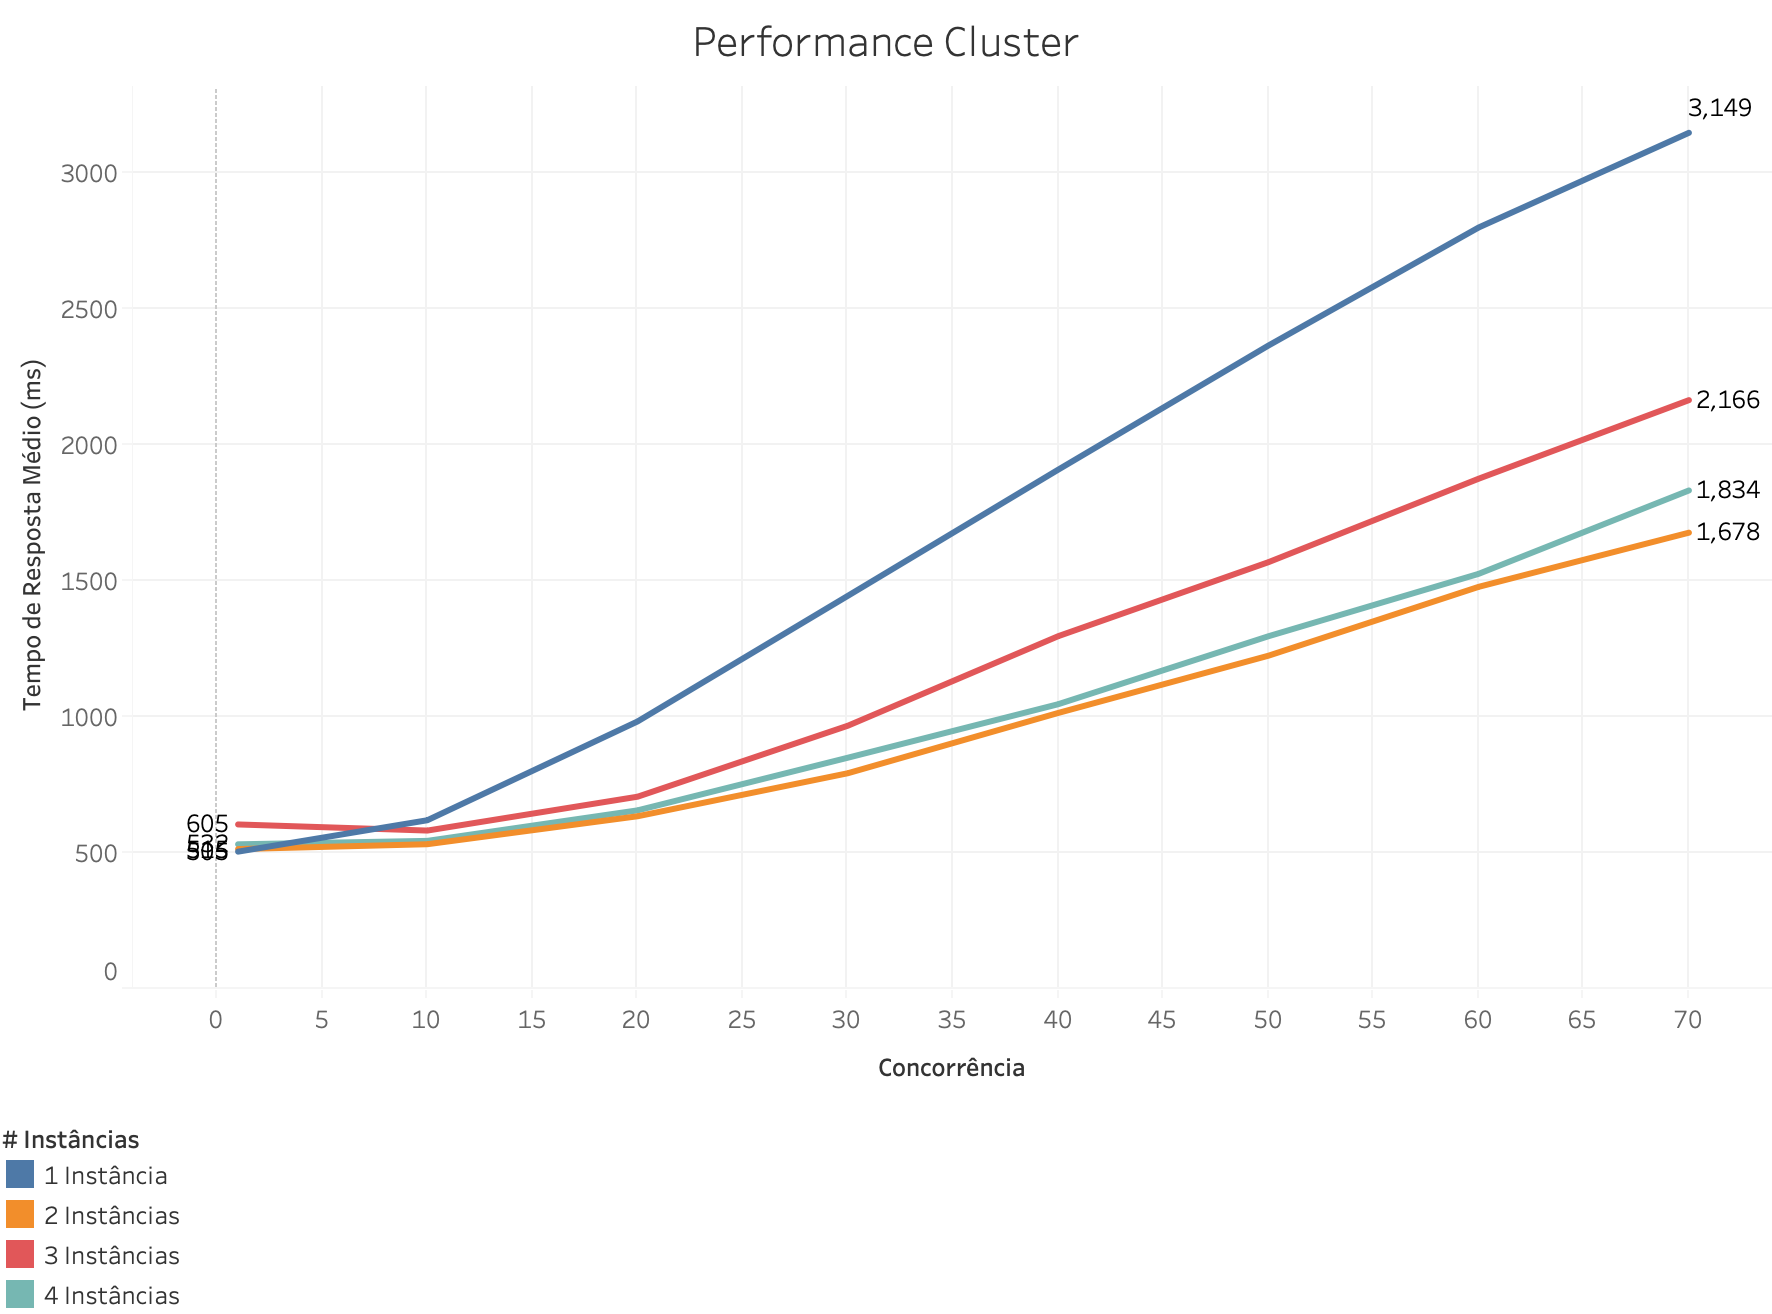
\includegraphics[width=8cm]{Imagens/Performance-Cluster}
    \caption{Tempo Médio de Resposta de Autenticação para Diferentes Tamanhos de \textit{Cluster}.}
    \label{fig.avg-resp-time-cluster}
\end{figure} 

Podemos observar nos resultados apresentados uma correlação positiva entre o nível de concorrência e o tempo médio de resposta do serviço independente da quantidade de instâncias disponíveis, comportamento similar ao apresentado na Figura \ref{fig.avg-resp-time}, onde testamos o \textit{Metabase} para uma única instância hospedado em um container \textit{Docker}. 

Já o efeito da escalabilidade na quantidade de instâncias resultou em uma melhora no tempo médio de resposta, no entanto, não de maneira linear como inicialmente esperava-se. Como podemos observar, os resultados obtidos para duas instâncias se apresentou melhor que os resultados da configuração com 4 instâncias que, por sua vez, se mostrou melhor que os resultados obtidos para 3 instâncias. 

\subsection{Experimento Comportamental}

Um segundo teste foi realizado com o intuito de analisar o comportamento da escalabilidade automática da quantidade de instâncias, por meio da ativação do \textit{horizontal pod autoscaler}. Conforme exposto na Seção 4, o HPA foi configurado para escalar a quantidade de instâncias quando o valor do percentual de uso médio da CPU das instâncias em execução ultrapassar 100\%, mantendo a quantidade de \textit{pods} entre 1 um 4. 

Esse teste consistiu na realização de 10 mil requisições ao serviço de autenticação com uma taxa de 60 requisições simultâneas. No estado inicial, existiam apenas um \textit{pod} em execução. 

Os resultados obtidos no teste de escalabilidade podem ser visualizados na Figura \ref{fig.avg-resp-time-hpa}, onde são apresentadas duas séries temporais, uma com o valor do tempo resposta (linha em cinza) e outra com a quantidade de instâncias em execução no momento (linhas coloridas, sendo azul para uma instância, amarelo para duas instâncias e vermelho para quatro instâncias).

\begin{figure}[htp]
   \centering
    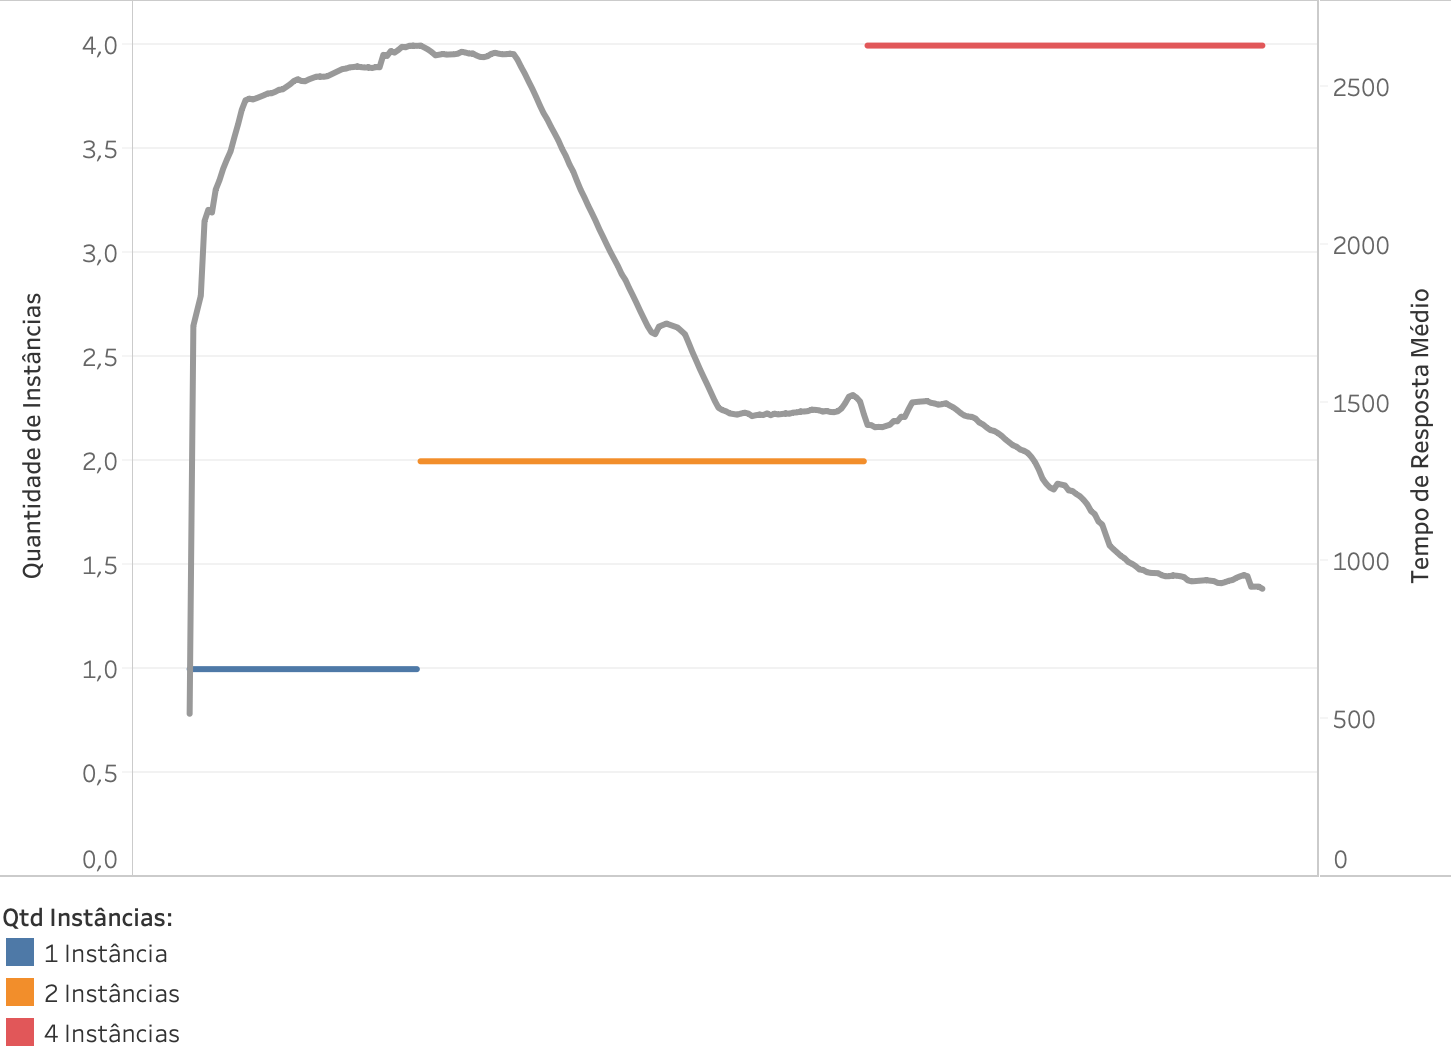
\includegraphics[width=8cm]{Imagens/Performance-HPA}
    \caption{Tempo Médio de Resposta de Autenticação com Escalabilidade Automática.}
    \label{fig.avg-resp-time-hpa}
\end{figure} 

Podemos observar, nitidamente, o decaimento no tempo de resposta a cada operação de \textit{scale-up} realizada no \textit{cluster}. Nota-se, também, um certo atraso no decaimento do tempo de resposta, que pode ser explicado pelo tempo entre a inicialização do Metabase, pois um \textit{pod} iniciado só passará a receber requisições do balanceador de carga no momento que o serviço estiver ativo.

Ainda analisando os resultados da Figura \ref{fig.avg-resp-time-hpa}, observamos que o decaimento no tempo de resposta quando o \textit{cluster} escala de duas para quatro instâncias não é tão representativo quanto o momento onde temos o crescimento de uma para duas instâncias. Este comportamento pode ser explicado quando analisamos novamente a figura \ref{fig.avg-resp-time-cluster}, e comparamos a distância entre as linhas de uma e duas instâncias em relação a distância entre as linhas de uma e quatro instâncias.


\subsection{Discurssão}

De uma maneira geral, os resultados apresentados nesta Seção indicam que a solução proposta atende aos objetivos deste trabalho, gerantindo um comportamento de escalabilidade automâtica do \textit{Metabase} por meio a implementação de um \textit{cluster} de instâncias. A medida que a demanda de uso do serviço aumentar, novos \textit{pods} serão instânciados e serão mantidos apenas enquanto necessário, provendo um melhor tempo de resposta e, consequentemente, uma melhor experiência para o usuário do sistema. 

Além disso, o conjunto de tecnologias utilizadas na solução adere perfeitamente aos planos de trabalho e de capacitação da Secretaria de Tecnologia, Informação e Comunição (STIC) do Tribunal Regional Eleitoral, o que facilita sua implantação e manutenção.

%Para melhor entendimento do comportamento observado a respeito da escalabilidade e definição de uma quantidade ótima de instâncias, seria necessário um estudo mais aprofundado quanto ao funcionamento do modelo de balancemento de carga, o que foje do escopo deste trabalho.